\subsection{Discrete-Event Trees}
\label{sec:MILP-selection-problem}
In this section we will derive algorithms for solving \eqref{eq:symbolic-optimization-with-minflow2} that are tailored to discrete-event trees.
For discrete event trees, the problem of the optimal scenario tree generation becomes one of selecting nodes from the original set of scenarios as nodes for the scenario tree.
It is generally possible to model the resulting selection problem as an MILP.
This full-size model, with far beyond 100,000 binary variables and a weak relaxation is, however, computationally intractable.

In the following section, an approach to overcome this complexity is discussed.
The model will be decomposed by time steps, each of which is still modeled as an MILP.
The model will be solved using a state-of-the-art mixed integer programming solver.
Some results on this method will be presented.
%
\subsubsection{Stage-Decomposition with MILP}
%
To reduce the complexity of the model, instead of solving all stages at the same time, we will solve the problem stage by stage.
This greatly reduces the computational burden, because using the filtration constraints, we can solve the branches of the tree one at a time.
These constraints allow us to
\begin{enumerate}
\item solve the branch starting from each of the previously fixed nodes independently.
\item for the current branch starting at node $j$, discard all scenarios $i$ for which $\eta_{ij}=0$ in the problem corresponding to the father node of $j$.
\end{enumerate}

The algorithm for solving the stage-wise tree construction problem will be presented in the following.
\begin{algorithm}
  % \SetAlgoLined
  \KwIn{Set $I$ of $T$-stage scenarios $\xi_i^t$, tree structure $\mathcal{T}$}
  \KwOut{Scenario tree consisting of nodes $\nu_n$ and probabilities $q_j$}
  $F \leftarrow \{1\}$\tcc*{init set of father nodes with root node}
  $S_1 \leftarrow I$\tcc*{All scenarios share the root node}
  \While{$F\neq \emptyset$}{
    \ForEach{$f\in F$}{
      $F \leftarrow F\setminus \{f\}$\tcc*{remove this node from father set}
      Solve the MILP $\mathcal{M}_{sw}(f)$\;
      \ForEach{$k\in \{j\in S_f | z_j^f=1\}$}{
        Set value of next child of $f$ to $\xi_k^t$\;
        $S_k \leftarrow \{i\in S_f| \eta_{ik}^f>0\}$\;
        \If{$k$ has children}{
          $F \leftarrow F\cup \{k\}$\;
        }
      }
    }
  }
  $q_j\leftarrow $ optimal weights \tcc*{Using Algorithm \ref{alg:optimal-weights}}
  \caption{Stage-Wise MILP based Scenario generation}
  \label{alg:stage-wise-milp}
\end{algorithm}
%At every branching point, algorithm \ref{alg:optimal-weights} performs the search for the $n_c$ scenarios that best cover the distribution given by all scenarios that the current node in the previous stage was used to cover.

The procedure is outlined as algorithm \ref{alg:stage-wise-milp}.
The input is a set of scenarios $I$ defined over a set of stages $T$ and a tree structure $\mathcal{T}$, typically defined by the number of branches of the tree at every node and time step.
The distances $c(\xi_i^t, \xi_j^t)$ between the scenarios $\xi_i,\,\xi_j\; i,j\in I$ can be computed beforehand.
Note that the $1$-norm is the only meaningful norm that can be constructed this way, since the full distance is implicitly approximated as a sum over the stages.
For consistency, $c$ should therefore be chosen as the $1$-norm.
Note that it is necessary to know the solution to the father node to be able to formulate the MILP $\mathcal{M}_{sw}(f)$ for a given node $f$.
A set $F$ is used to keep track of the nodes for which can be solved next.
This set is initialized with the root node of the tree.
Additional sets $S_f\subset I$ are introduced for all $f\in F$.
These sets hold all scenarios of the scenario set $I$ that are associated with the node $f$ through the transport variables $\eta$.
Only the scenarios that had a non-zero ``mass-flow'' $\eta$ in the Kantorovich functional evaluation of their father node will be used in the construction of node $f$'s children in the tree.
This property preserves the filtration information in the stage-wise algorithm.

The problem that is solved for each father node $f$ in the previously defined tree is the following MILP:
\begin{eqnarray} % besser align?
  \label{eq:small-milp-in-alg}
  \mathcal{M}_{sw}(f)\; \; \min_{\eta^f,z^f}&&\sum_{i\in I_f}\sum_{j\in I_f}\eta_{ij}^fc(\xi_i^t,\xi_j^t)\\
  \mathrm{s.t.}&&\sum_{j\in I_f}\eta_{ij}^f = \eta_{if}^{father(f)}\\
  &&\sum_{j\in I_f}z_j^f \leq n_c^f\\
  \label{eq:1}
  &&\eta_{ij}^f\leq z_j^f\\
  &&0\leq \eta_{ij}^f\\
  &&z_j^f\in\left\{0,1\right\}
\end{eqnarray}
The MILP models the decision which scenarios will be selected as nodes into the tree.
The variables $z_j^f$ are the selection variables for the scenarios $\xi_j$.
If the node $\xi_j^t$ of scenario $j$ at time step $t$ (which is the time step following the current father node $f$) is selected as a node of the tree, the corresponding selection variable is set to $z_j^t=1$.
Only $n_c$ (number of children, determined by the tree structure) nodes may be selected.
The inequality constraints \eqref{eq:1} ensure that there are no flows $\eta$ directed to nodes that were not selected.

Note that this problem has the worst possible relaxation. The LP solution without integrality constraints is
\begin{align}
  \label{eq:2}
  z_j^t &= \eta_j^{father(f)}\\
  \eta_{ij} &= \left\{
    \begin{array}{ll}
      \eta_j^{father(f)}&\text{if } i=j\\
      0&\text{otherwise}
    \end{array}
  \right.\\
  \sum_{i\in I_f}\sum_{j\in I_f}\eta_{ij}^fc(\xi_i^t,\xi_j^t) = 0
\end{align}

Figure \ref{fig:swmilp-explanation} shows the evolution of the algorithm.
\begin{figure}
\centering
  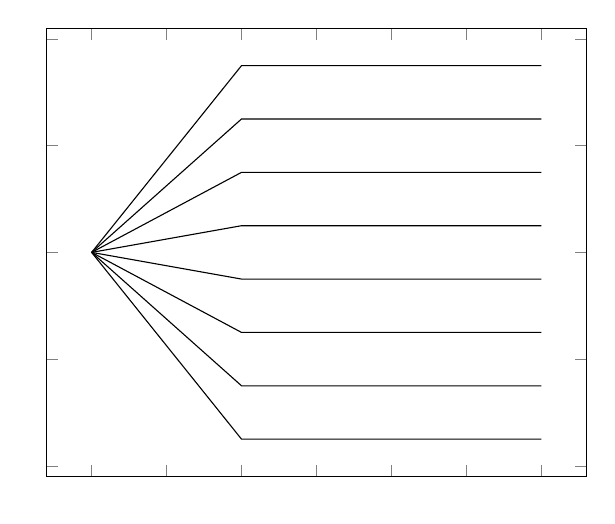
\begin{tikzpicture}
    \begin{axis}[xticklabels={,,},yticklabels={,,}]
      \addplot [color=black] coordinates {
        (1, 0)
        (2, -3.5)
        (3, -3.5)
        (4, -3.5)
      };
      \addplot [color=black] coordinates {
        (1, 0)
        (2, -2.5)
        (3, -2.5)
        (4, -2.5)
      };
      \addplot [color=black] coordinates {
        (1, 0)
        (2, -1.5)
        (3, -1.5)
        (4, -1.5)
      };
      \addplot [color=black] coordinates {
        (1, 0)
        (2, -0.5)
        (3, -0.5)
        (4, -0.5)
      };
      \addplot [color=black] coordinates {
        (1, 0)
        (2, 0.5)
        (3, 0.5)
        (4, 0.5)
      };
      \addplot [color=black] coordinates {
        (1, 0)
        (2, 1.5)
        (3, 1.5)
        (4, 1.5)
      };
      \addplot [color=black] coordinates {
        (1, 0)
        (2, 2.5)
        (3, 2.5)
        (4, 2.5)
      };
      \addplot [color=black] coordinates {
        (1, 0)
        (2, 3.5)
        (3, 3.5)
        (4, 3.5)
      };
    \end{axis}
  \end{tikzpicture}
  % begin of figure 2
  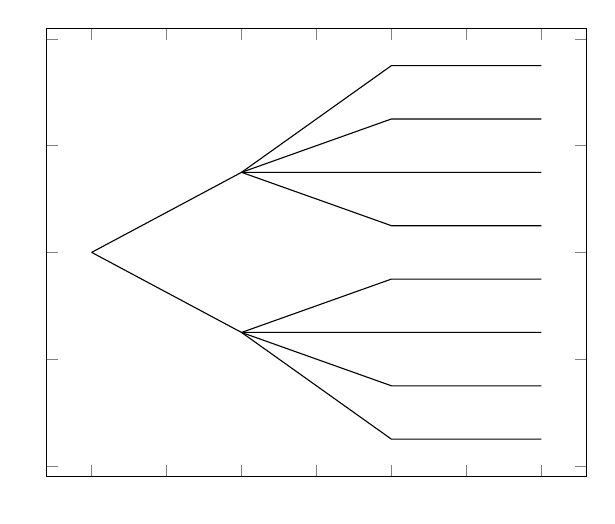
\begin{tikzpicture}
    \begin{axis}[xticklabels={,,},yticklabels={,,}]
      \addplot [color=black] coordinates {
        (2, -1.5)
        (3, -3.5)
        (4, -3.5)
      };
      \addplot [color=black] coordinates {
        (2, -1.5)
        (3, -2.5)
        (4, -2.5)
      };
      \addplot [color=black] coordinates {
        (1, 0)
        (2, -1.5)
        (3, -1.5)
        (4, -1.5)
      };
      \addplot [color=black] coordinates {
        (2, -1.5)
        (3, -0.5)
        (4, -0.5)
      };
      \addplot [color=black] coordinates {
        (2, 1.5)
        (3, 0.5)
        (4, 0.5)
      };
      \addplot [color=black] coordinates {
        (1, 0)
        (2, 1.5)
        (3, 1.5)
        (4, 1.5)
      };
      \addplot [color=black] coordinates {
        (2, 1.5)
        (3, 2.5)
        (4, 2.5)
      };
      \addplot [color=black] coordinates {
        (2, 1.5)
        (3, 3.5)
        (4, 3.5)
      };
    \end{axis}
  \end{tikzpicture}
  % begin of figure 3
  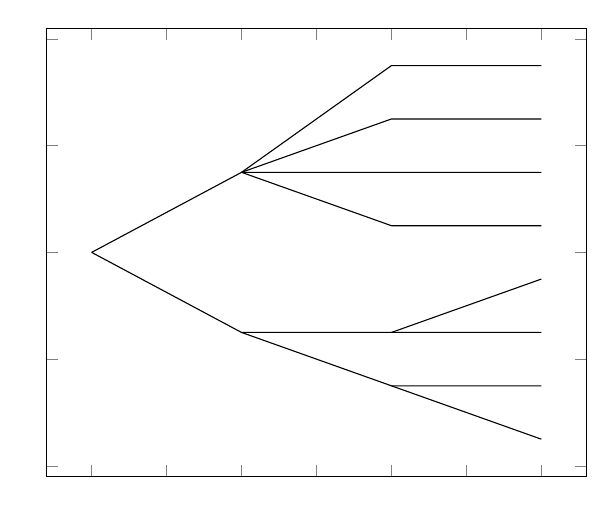
\begin{tikzpicture}
    \begin{axis}[xticklabels={,,},yticklabels={,,}]
      \addplot [color=black] coordinates {
        (3, -2.5)
        (4, -3.5)
      };
      \addplot [color=black] coordinates {
        (2, -1.5)
        (3, -2.5)
        (4, -2.5)
      };
      \addplot [color=black] coordinates {
        (1, 0)
        (2, -1.5)
        (3, -1.5)
        (4, -1.5)
      };
      \addplot [color=black] coordinates {
        (3, -1.5)
        (4, -0.5)
      };
      \addplot [color=black] coordinates {
        (2, 1.5)
        (3, 0.5)
        (4, 0.5)
      };
      \addplot [color=black] coordinates {
        (1, 0)
        (2, 1.5)
        (3, 1.5)
        (4, 1.5)
      };
      \addplot [color=black] coordinates {
        (2, 1.5)
        (3, 2.5)
        (4, 2.5)
      };
      \addplot [color=black] coordinates {
        (2, 1.5)
        (3, 3.5)
        (4, 3.5)
      };
    \end{axis}
  \end{tikzpicture}
  % begin of figure 4
  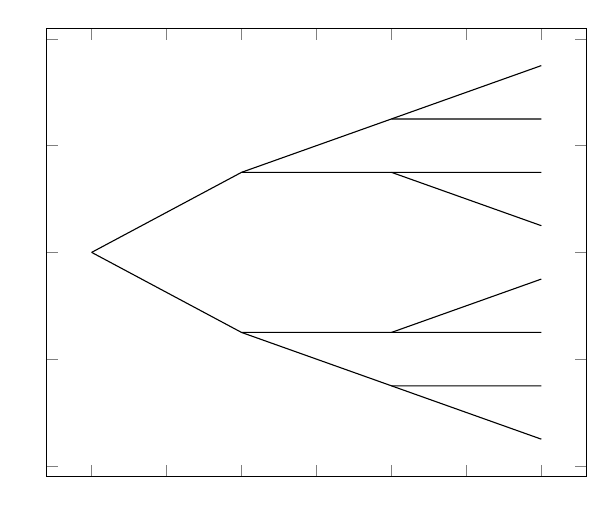
\begin{tikzpicture}
    \begin{axis}[xticklabels={,,},yticklabels={,,}]
      \addplot [color=black] coordinates {
        (3, -2.5)
        (4, -3.5)
      };
      \addplot [color=black] coordinates {
        (2, -1.5)
        (3, -2.5)
        (4, -2.5)
      };
      \addplot [color=black] coordinates {
        (1, 0)
        (2, -1.5)
        (3, -1.5)
        (4, -1.5)
      };
      \addplot [color=black] coordinates {
        (3, -1.5)
        (4, -0.5)
      };
      \addplot [color=black] coordinates {
        (3, 1.5)
        (4, 0.5)
      };
      \addplot [color=black] coordinates {
        (1, 0)
        (2, 1.5)
        (3, 1.5)
        (4, 1.5)
      };
      \addplot [color=black] coordinates {
        (2, 1.5)
        (3, 2.5)
        (4, 2.5)
      };
      \addplot [color=black] coordinates {
        (3, 2.5)
        (4, 3.5)
      };
    \end{axis}
  \end{tikzpicture}
  \caption{Evolution of the stage-wise MILP algorithm for a tree with two branches to each node.
    Top left: The tree is initialized with only the root node.
    Top right: After solving the MILP of the root node.
    Bottom left: After solving the lower of the two second stage nodes.
    Bottom right: The tree, completely solved.
  }
  \label{fig:swmilp-explanation}
\end{figure}
%%% Local Variables:
%%% mode: latex
%%% TeX-master: "da"
%%% End:
 % figure fig:swmilp-explanation

The results of this algorithm applied to a small problem will briefly be discussed.
For a test problem, a geometric brownian motion based on $\mathcal{N}(0,0.5)$ was used.

The first important question was whether using this elaborate approach yields considerably better results than the naive approach of sampling the tree nodes directly from the original distribution.
This question is answered positively in figure \ref{fig:naive-milp-results-errors}.
Even for this very regular problem, the error for the random solution was twice as high as that of the optimal solution.
However, the run time proved to be the main drawback of this algorithm.
Run times for the geometric brownian motion with different numbers of sampled scenarios are plotted in figure \ref{fig:naive-milp-results-timing}.
Eve though the state-of-the-art solver Gurobi 4.01 was used, problems with 2000 sampled scenarios could not be solved on a dual core 2500Mhz processor with 4 GB RAM.
\begin{figure}
  \centering
  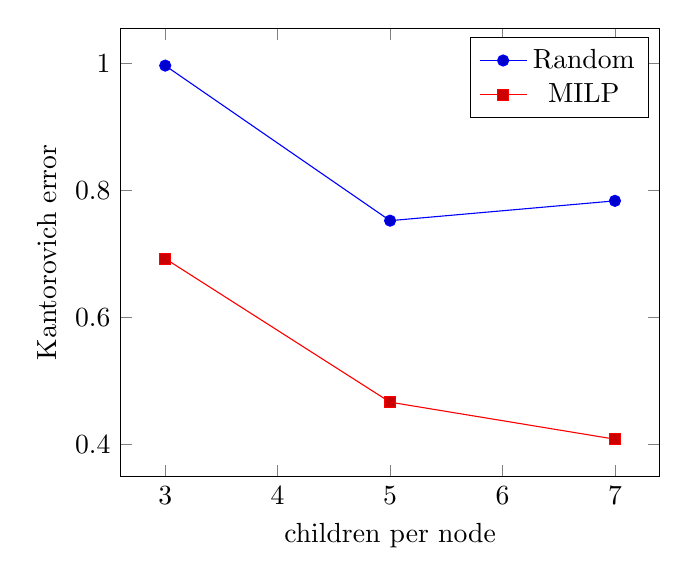
\begin{tikzpicture}
    \begin{axis}%[error bars/y explicit]
      [
      legend entries={Random,MILP},
      xlabel=children per node,
      ylabel=Kantorovich error
      ]
      \addplot  coordinates { % random selection (ultra-naive algorithm)
        (3, 0.9967) %+ (0,0.2379) - (0,0.1479)
        (5, 0.7525) %+ (0,0.1338) - (0,0.0830)
        (7, 0.7837) %+ (0,0.1562) - (0,0.0697)
      };
      \addplot coordinates { % stage-wise MILP
        (3, 0.6927)
        (5, 0.4667)
        (7, 0.4084)
      };
    \end{axis}
    \end{tikzpicture}
  \caption{Results for the stage decomposition algorithm using an MILP solver for each stage for different numbers of children/branches. Number of stages: $n_s=3$, stochastic process: geometric brownian motion, initial value 1, $\mu=0,\,\sigma=0.5$}
  \label{fig:naive-milp-results-errors}
\end{figure}
\begin{figure}
  \centering
  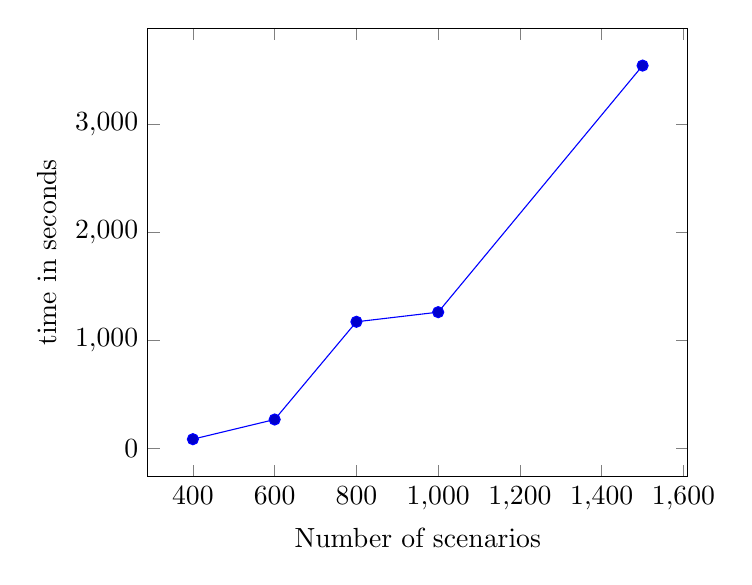
\begin{tikzpicture}
    \begin{axis}
      [xlabel=Number of scenarios, ylabel=time in seconds]
      \addplot coordinates{ % Timing
        (400, 85.1)
        (600, 267.4)
        (800, 1172.9)
        (1000, 1261.9)
        (1500, 3546.5)
      };
    \end{axis}
  \end{tikzpicture}
  \caption{Results for the stage decomposition algorithm: Run times in seconds over the number of scenarios of the initial distribution. At 2000 scenarios, the algorithm failed on 4GB RAM due to memory problems.}
  \label{fig:naive-milp-results-timing}
\end{figure}
%%% Local Variables:
%%% mode: latex
%%% TeX-master: "da"
%%% End:

%%% Local Variables:
%%% mode: latex
%%% TeX-master: "da"
%%% End:
